\section{Repair in Parametric Space}
\label{sec:repair}

Flattening the sheet turns CT read-back into a repair instrument. Defects that are ambiguous on the folded surface become local evidence in the developed domain: a delaminated double layer covers the same $(u,v)$ twice; an off-sheet prediction is a dark island surrounded by papyrus texture; a bad atlas seam breaks a fibre that should continue. These operations are organized in the parametric domain, but they can update either 3D geometry (overlap selection and snap) or only UV coordinates (registration and relaxation). They complement the mesh-space repairs of Section~\ref{sec:cleanup}, which establish connectivity before image evidence is consulted.

\paragraph{Separating delaminated layers.} Where the papyrus has physically split into two nearly-coincident plies, the earlier geometric split cannot always tell them apart, and they arrive at the same $(u,v)$ and blur together in the read-back. Separating them is a two-energy problem. First we partition the multiply-covered region's triangles into layers with a lifted multicut~\cite{keuper2015efficient}: triangles adjacent in $(u,v)$ are joined by an {\em attractive} edge whose weight is their shared parametric edge length, while triangles that overlap at the same $(u,v)$ but lie far apart in 3D --- the delamination cue --- are joined by a strongly {\em repulsive} lifted edge. Minimizing the multicut objective
\begin{equation*}
  E_{\mathrm{cut}} = \!\!\sum_{(i,j)\,\mathrm{adj}}\!\! w_{ij}\,[\ell_i \neq \ell_j] \;+\!\! \sum_{(i,j)\,\mathrm{ovl}}\!\! |w_{ij}|\,[\ell_i = \ell_j]
\end{equation*}
over triangle labels $\ell$ (Kernighan--Lin, at least two clusters) keeps a connected ply together while forcing the two overlapping sheets onto different labels. Second, we decide which ply to keep with a {\em quilting energy}, the min-error boundary of image quilting~\cite{efros2001image}: we raster the CT intensity of each candidate ply and of the surrounding clean {\em anchor} sheet, and score the ply by the mean intensity discontinuity along their shared seam,
\begin{equation*}
  E_{\mathrm{quilt}} = \frac{1}{|\partial|}\sum_{p \in \partial} \bigl| (v^{L}_p - \bar v^{L}) - v^{A}_p \bigr|,
\end{equation*}
where $\partial$ are the seam-adjacent pixels and $\bar v^{L}$ removes any per-ply brightness offset. Because papyrus is near-uniform in mean brightness, $E_{\mathrm{quilt}}$ is dominated by whether the fibre pattern {\em lines up} across the seam; we keep the substantial ply that minimizes it --- the one whose texture best continues the surrounding sheet --- and relocate it to its own place in the atlas.

\paragraph{RAW-guided surface snap.} The U-Net occasionally places a surface patch in a dark inter-sheet gap rather than on papyrus (Fig.~\ref{fig:snap}, top). Snap is a current production stage, though its target objective is still being refined. A contrast-sensitive binary graph cut~\cite{boykov2001fast} first labels dark and supported vertices in the developed texture. For each dark island, samples are taken at signed depths along a stable across-sheet radial direction. A geometric occupancy query excludes the island's own neighbourhood and stops a ray before it enters any other mesh, so no candidate can cross an intervening wrap. An island without a supported boundary or an admissible free-space target remains an anchor and is not moved.

The first repair pass chooses target depths {\em jointly}, not as independent intensity maxima. Candidate positions for vertex $i$ are sampled at an odd number of signed depths $d_i$ along its across-sheet radial direction; the data cost $Q_i(d_i)=|v_{\mathrm{RAW}}(i,d_i)-\bar v_i|$ is the quilting mismatch between the RAW intensity sampled at that depth and the clean-boundary intensity $\bar v_i$ propagated inward from the island's nearest supported rim, so a candidate is cheap exactly when it {\em continues} the surrounding papyrus signal. A displacement penalty $\alpha|d_i|$ prefers small moves, and neighbouring labels pay a truncated-linear discontinuity cost,
\begin{equation*}
 E_{\mathrm{snap}}(d)=\sum_i \bigl(Q_i(d_i)+\alpha |d_i|\bigr)
 +\lambda\!\sum_{(i,j)\in E}\!\min\!\left(\tau,|d_i-d_j|\right),
\end{equation*}
which is optimized by alpha expansion (weights in Appendix~\ref{app:terms}). A zero-displacement label is always available, and a vertex with no legal target is forced to it, so unfixable vertices double as barriers that stop a target field from jumping to the far side of a sheet. The selected targets drive a screened-Laplacian displacement solve with clean vertices pinned. Solved vertices that violate occupancy are reverted. The purpose of the quilting term is coherence: a repaired island should continue the surrounding fibre pattern rather than chase whichever bright voxel happens to be nearest.

A second, global {\em recto refinement} addresses the fact that papyrus placement is not an intensity-maximum problem. Along the outward line it searches for an oriented dark-to-bright RAW transition, scores the transition with a local tangent-tensor quality estimate, and solves a smooth scalar displacement field over the mesh. Unsupported regions remain anchored; Jacobi updates, slope limits, damping, occupancy tests, and per-vertex reversion keep the pass conservative. This second objective is currently under real-data A/B evaluation. It improves the physical meaning of the target, but snap is not yet perfect in the crumpled core and is reported as such rather than omitted from the pipeline.

\begin{figure}[t]
  \centering
  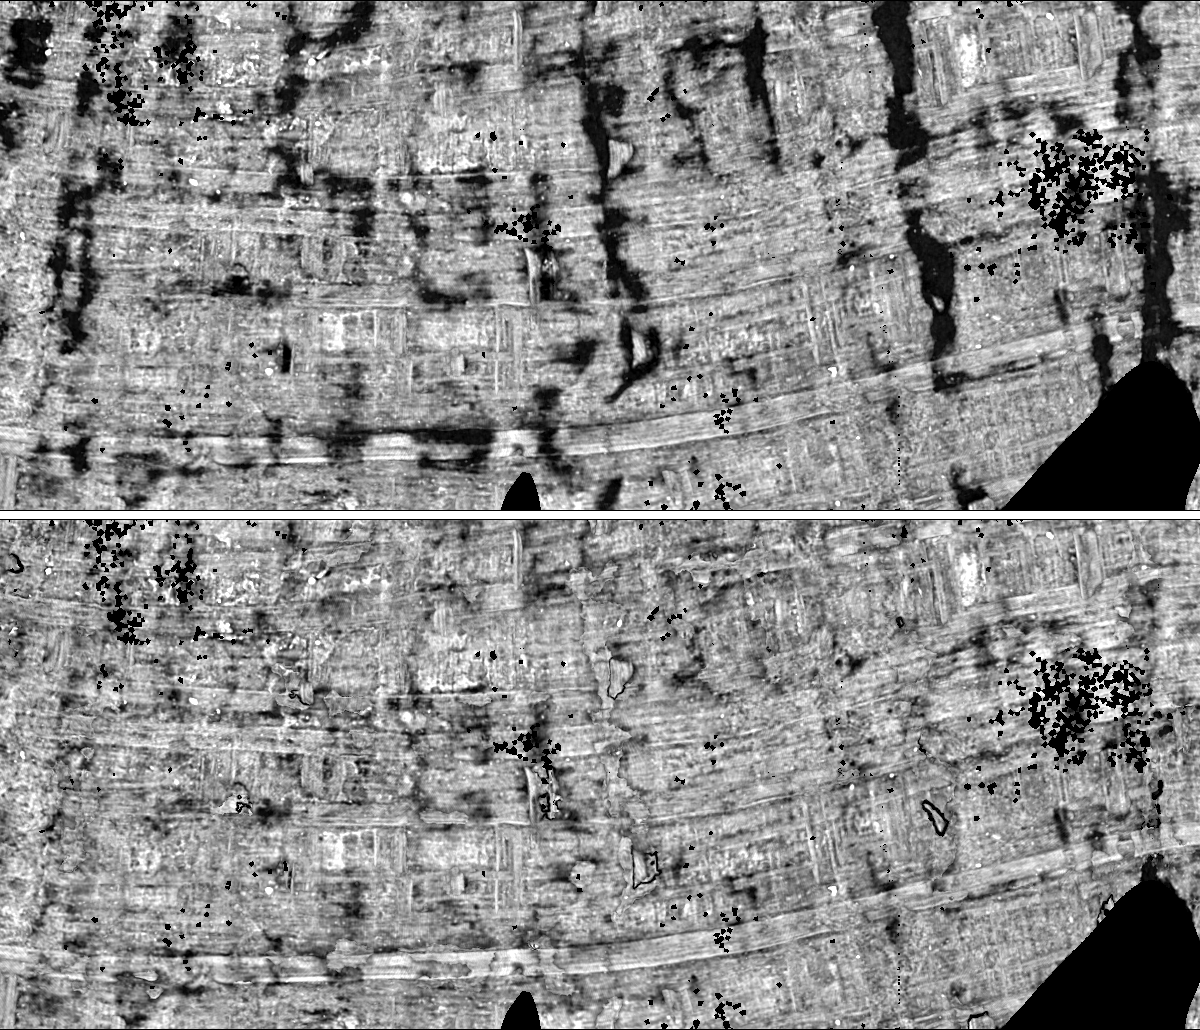
\includegraphics[width=\linewidth]{figures/snap_beforeafter.png}
  \caption{RAW-guided off-sheet repair, before (top) and after (bottom), on one developed region. Dark islands with supported boundaries are assigned coherent, occupancy-safe target depths and moved by a smooth solve. Persistent dark speckle is left in place when the evidence indicates real cracks or supplies no safe target.}
  \Description{Two grayscale CT texture crops. The lower repaired crop has more continuous bright papyrus texture while isolated dark cracks remain.}
  \label{fig:snap}
\end{figure}

\paragraph{Parameter-domain finalization.} After geometry repair, neighbouring ribbons are welded in UV and a quilting-based registration warp corrects residual $u$ offsets while preserving the established winding. The optional in-house relaxation combines symmetric Dirichlet distortion~\cite{smith2015bijective} with a fibre-alignment term derived from the structure tensor~\cite{bigun1987optimal}, and rejects any step that flips a triangle. It remains an experimental diagnostic: in the verified-patch test it worsened mean stretch and left flips, so the accepted local workflow delegates final flattening to Villa. For whole-scroll atlases, only registration candidates that improve seam mismatch and preserve coordinate validity are retained.

\paragraph{Collision-safe ribbon fitting.} The winding lift decides {\em which} wind each chart occupies; what remains is to turn the registered atlas into a single ribbon whose rows do not pass through one another. We slice the placed geometry at constant $v$ and sample each row at a common $u$ isovalue spacing, recording for every sample its position and unit tangent in the plane normal to the scroll axis. Samples that coincide in 3D within a local tolerance {\em and} agree in tangent are merged; those that coincide but disagree are recorded as conflicts rather than averaged, because a disagreeing tangent is the signature of two different wraps, not of noise. Each row is then fitted on a coarser control spacing by a least-squares problem combining observation position, a zero-curvature smoothness term, and a tangent term that integrates unit progress in $u$ (weights in Appendix~\ref{app:terms}). Where a row has no support, a bridge is admitted only if its chord is metrically plausible: a chord longer than $1.25\,\Delta u$ plus a small slack is rejected outright, on the principle that a metrically impossible bridge is evidence of a topology error and not a gap to be filled.

The fitted rows are then registered by smoothing each chart's $U$ shift along $v$, and finally audited for collision {\em exactly}. Rather than scoring occupancy on a grid, each round runs exact pairwise tests between rows and applies a fixed fraction of the computed escape, repeating until the ledger stops improving; an optional pass aligns the phase of adjacent rows against the RAW texture. This is the terminal stage of the whole-scroll path, and like the winding lift it reports its residual overlaps instead of declaring the surface verified.

Every fitted edge that is absent carries the gate that removed it. Measured on a default end-to-end run of the $4\times5\times5$ fixture --- stock parameters throughout, not the tuned winding campaign reported above --- the ribbon carries 9.1\% of the observed atlas area; the audit attributes the remainder to unbridgeable $u$ gaps (40.7\%), the vertical metric cut (26.9\%), topology cuts (19.4\%), and the horizontal metric cut (2.5\%), with rows outside the $v$ lattice, absent $u$ support, sub-grid islands, crossings, and geometry mismatch together accounting for the final 1.4\%. We report the breakdown rather than the single number because the reasons are actionable in a way the fraction is not: a $u$ gap is missing atlas, whereas a topology cut is the ribbon declining to bridge two wraps, and only the first is a coverage problem. A hole here is auditable evidence about the underlying atlas, not a silent omission.

